\chapter {In-Situ Formation of STIPs}

%Intro outline:
% What are STIPs, why important
% Outline of formation theories, migration vs in-situ
% Problems with migration models, in-situ simpler
% Outline my previous paper
% Motivation: does accretion boundary leave any imprint on final orbital architectures?

\section{Introduction} \label{sec:intro}

One of the most surprising and intriguging results from NASA's \textit{Kepler} mission was the prevalance 
of sub-Neptune-sized exoplanets with orbital periods shorter than that of Mercury \cite{borucki10}. These 
planets are often found in closely-spaced groups, known as systems of tightly-packed inner planets (
STIPs) \cite{latham11, lissauer11, lissauer14}. STIPs are found to often be coplanar 
\cite{fang12, tremaine12}, have low eccentricities \cite{vaneylen15, hadden17} and are usually not in 
mean-motion resonance with each other \cite{fabrycky14, steffen15}. In addition these systems have been 
shown to exhibit a compelling amount of uniformity between adjacent planets, in terms of mass, radius and 
orbital spacing \cite{millholland17, millholland21}.

All of these characteristics provide a rich set of constraints for planet formation models. One of the 
most intriguing questions that arises is why the structure of the present-day solar system appears so 
different than that of STIPs. Extending the minimum-mass solar nebular (MMSN) model \cite{hayashi81} down 
to $\sim$ 0.05 AU, where the inner edge of many protoplanetary disks are thought to be \cite{meyer97} (
and where planetesimals are thought to form \cite{mulders18}) yields several extra Earth masses of 
material. Explaining why this material is missing from the solar system, but not some exoplanetary 
systems, is a key question that a complete theory of planet formation must be able to provide.

There are two categories of formation theories meant to explain the ubiquity of these compact, short-period systems. The first 
involves the gradual assembly of these worlds as they migrate inwards. For Mars-sized bodies and larger, torques at the Lindblad 
resonances drive the exchange of angular momentum between the gaseous disk and the planet \cite{ward97}. A key prediction of 
migration models is that multiplanet systems should end up in resonant chains \cite{cresswell06}. Although this is not unheard of 
(see Kepler 223 \cite{mills16} and Trappist-1 \cite{gillon16, gillon17, agol21}), the majority of these systems are found to not be in 
resonant chains \cite{lissauer11, fabrycky14}. One potential explanation for this discrepancy involves a later phase of 
destabilization after convergent migration has completed and the gaseous disk subsequently dissipates 
\cite{izidoro17, izidoro21}. However, the detailed behavior of tidal torque-driven migration is still very uncertain and it is not 
entirely clear when and how convergent migration should operate. The strength and even direction of tidal migration depends 
sensitively on the thermodynamic structure of the gas disk \cite{ayliffe10, bitsch13}.

Alternatively, these planets may have formed in situ, having been constructed only from the local mass budget of the disk. This 
appears to be the case for the gaseous envelopes of hot Jupiters formed near the inner edge of the disk \cite{bailey18}, although 
it is not clear whether the cores of these worlds require a migration model. Currently, there are no measurements constraining the 
mass budget of the innermost regions of planet-forming disks, so the initial conditions for in situ models tend to rely on wild 
speculation. By enhancing the solid surface density by a factor of $\sim$ 100 relative to the inner solar system, \cite{hansen12} 
was able to form compact multiplanet super-Earth systems without invoking any kind of planet migration. In situ formation may be 
particularly prevalent around low mass stars, as magnetically-driven disk winds tend to flatten out the radial gas density profile, 
which balances out the inner and outer torques from tidally-driven migration \cite{ogihara18}. One should note that no in situ 
models have yet to produce resonant chains of planets, so it seems likely that gas disk migration likely plays a role at least for the 
subset of planetary systems found in this type of configuration.

Compared to planet formation models that involve gas disk-driven migration, an in situ model is relatively straightforward 
(although expensive) to model, involving only mutual gravitational interactions and the occasional collision. In (Wallace + Quinn 
2023, cite once published), we used a tree-based N-body code to follow the accumulation of near realistic-sized planetesimals 
into protoplanets at short orbital period. We showed that oligarchic growth \cite{kokubo98}, which gives rise to a bimodal 
population of protoplanets and residual planetesimals, does not operate at arbitrarily short orbital periods. In addition, the 
boundary between oligarchic and non-oligarchic growth should be expected to lie somewhere in the middle of a typical STIP.

In this work, we use a hybrid symplectic N-body code to grow the protoplanet systems from (Wallace + Quinn 2023, cite once 
published) to completion. These comprise the first ever end-to-end N-body simulations that directly follow the growth of the 
smallest gravitational aggregates to full-sized terrestrial planets. In section \ref{sec:simulations}, we describe the simulation code 
we use, along with how previous protoplanet simulations are used to construct the initial conditions for the final assembly phase. In 
section \ref{sec:results}, we examine the final orbital architectures of the simulated STIPs, and investigate whether the accretion 
mode boundary persists in any measurable way. In section \ref{sec:typicalICs}, we compare our results with a set of simulations 
run starting with a more `typical' distribution of fully-formed, evenly spaced protoplanets and show that a more self-consistent 
treatment tends to result in a subset of systems undergoing a potentially destructive phase in the inner disk. Due to the 
stochasticity of our results, we use the simulation snapshots from (Wallace + Quinn 2023, cite when published) to train a neural 
network to produce an infinite set of qualitatively similar, but numerically distinct initial conditions and then compare these with the 
full simulation runs in section \ref{sec:neuralICs}. Finally, we conclude in section \ref{sec:discuss} and discuss whether the absence 
of any short-period planets in the solar system might point toward a largely in situ formation history.

% Plots to make:
% 1 A summary of the initial conditions from the ChaNGa simulations, period-ecc, period-mass
% 2 time-Period plot of ChaNGa-genga simulations (full page?) with collisions overlaid
% 3 period-mass for final genga snapshots for each surface density profile
% 4 composition plots with arbitrary snowline for final genga snapshots
% 5 period-mass and period-ecc plots for full genga and iso sims
% 6 composite time-period plot for all collisions in full changa+genga and iso sims
% 7 collision speed plots for full changa+genga and iso sims
% 8 plot planetary architectures with markers for destroyed planets, full changa+genga and iso sims
% 9 diagram explaining how GAN model works
% 10 corner plot showing training and synthetic data
% 11 sdv data quality plots
% 12 period-mass and period-ecc plots comparing changa+genga full sims and synthetic sims
% 13 time-period plot for changa+genga full sims and synthetic sims
% 14 corner plot comparing rmc, amd, mean_ecc and n_pl for full sims, syntheic sims and iso sims
% 15 collision speed plots for full changa+genga and synthetic sims
% 16 plot planetary architectures with markers for destroyed planets, full changa+genga and synthetic sims

\section{Simulations} \label{sec:simulations}

\subsection{Numerical Methods} \label{sec:numerical}

A direct N-body model of the full collisional evolution of a system of terrestrial planets, starting from planetesimals, covers over 
6 orders of magnitude in mass growth. Although main physics drivers are gravity and solid body collisions, the wide range of 
timescales that must be resolved during the accretion process necessitate the use of a multi-phase integration scheme. Early 
on, interactions between planetesimals are frequent and encounter timescales can be as short as $\sim$ hours (check this). 
As planetary embryos form, the timescale for gravitational instability can lengthen to $10^{5}$ years \cite{chambers96}, while 
the final planet assembly process can take Myrs. For traditional N-body codes that use a leapfrog integrator, Myr integrations 
of a planetary system require $\sim 10^{10}$ timesteps, which is prohibitively long for even the most modest resolutions. To 
circumvent this problem, a hybrid mixed variable symplectic (MVS) scheme \cite{chambers99} can be used, which greatly 
reduces the number of timesteps required so long as close encounters are extremely infrequent.

However, close encounters are certainly frequent during the planetesimal accretion process, and so a hybrid MVS scheme is 
not appropriate here. To properly resolve the planetesimal accretion process, while still being able to integrate the planet 
formation process to completion, we split our simulations into two separate phases. In the first phase, we track planetesimal 
growth using the highly parallel N-body code {\sc ChaNGa}. Gravitational forces are calculated using a modified Barnes-Hut 
\cite{barnes86} tree with hexadecapole expansions of the moment. For all of our simulations, we use a node opening criterion 
of $\Theta_{BH}$ = 0.7. The equations of motion are integrated using a kick-drift-kick leapfrog scheme and collisions are 
treated as solid spherical bodies which produce a complete and instantaneous merger. A more complete description of  
{\sc ChaNGa} can be found in \cite{jetley08, menon15} and a description of the collision detection and resolution module, 
which is largely based off of the implementation in PKDGRAV \cite{richardson94, richardson00}, can be found in 
\cite{wallace19}.

As the particle count diminishes and the encounter timescales lengthen, the final simulation snapshots from {\sc ChaNGa} are 
passed to the hybrid MVS code {\sc genga} \cite{grimm14, grimm22}. Like {\sc mercury} \cite{chambers99}, {\sc genga} splits 
the Hamiltonian into a Keplerian and perturbing part and solves these independently using a mixed variable symplectic 
scheme. For close encounters, the perturbing part of the Hamiltonian becomes large and a Bulirsch-Stoer integrator takes over 
to update the equations of motion for these particles. To permit larger close encounter groups, a heirarchical method with 
multiple changeover functions is used, which acts to break the close encounters into multiple subgroups which can be 
integrated independently. All of this work is done on GPU hardware, and can be done with up to 60,000 particles while running 
up to 30x faster than {\sc Mercury}. For all of the {\sc genga} simulations presented in this work, we use a maximum subgroup 
size of 512 particles and allow for 2 substeps on each level of the changeover function.

\subsection{Initial Conditions} \label{sec:ics}

Each simulation begins with an equal-mass disk of planetesimals with $m_{pl} = 5 \times 10^{22}$ g and $\rho_{pl} = 3$ g cm$^{-3}$ orbiting a 0.08 $M_{\odot}$ star. Semimajor axes of the bodies are randomly drawn between 1 and 100 days in orbital period such that the mass surface density profile follows

\begin{equation}
	\Sigma(r) = \textrm{10 g cm}^{-2} \times A \left( \frac{M_{*}}{M_{\odot}} \right) \left( \frac{r}{\textrm{1 AU}} \right)^{-\delta}
\end{equation}
where $M_{*}$ is the mass of the central star, 10 g
cm$^{-2}$ is the surface density of the minimum-mass solar nebula
\cite[MMSN]{hayashi81} at 1 AU, $A$ is an enhancement factor and $\delta$ is the power law index. Following \cite{hansen12} we use $A = 100$. To test the influence that the surface density profile has on the final planet configuration, we use $\delta$ = 0.5, 1.5 and 2.5. 

Due to the stochasticity of the final assembly phase, we generate 5 distinct initial conditions with each configuration, each using a different random number seed. In all cases, the eccentricities and inclinations are drawn from a Rayleigh distribution with $\left< e^{2} \right>^{1/2} = 2\left<i^{2} \right>^{1/2} = e_{eq}$ \cite{ida93}. The eccentricity dispersion is set such that the viscous stirring timescale is in balance with the aerodynamic gas drag timescale. In both phases of the simulations, the gas surface density is a factor of 240 times larger than the solid surface density, and a power law index of 1.5 is used, even in the cases where the profile of the solids is steeper or shallower than this. In addition to being used to construct the initial conditions, the prescribed gas profile is used to apply a Stokes drag force to the growing planetesimals and protoplanets.

To make the planetesimal accretion phase more computationally tractable, the collision cross sections of particles are inflated by a factor of 6. This acts to shorten the growth timescale and number of timesteps required to produce protoplanets without qualitatively changing the growth modes. The collision cross section inflation, however, does move the boundary between oligarchic and non-oligarchic growth in the disk outward by a factor of $\sim$ 10 in orbital period. In figure \ref{fig:changa_ics}, we show the eccentricity and mass distribution at the end of the planetesimal accretion phase for a simulation using $\delta$ = 1.5. For a full description of how the initial conditions were constructed, along with the details of the simulations and the limitations created by expanding the collision cross sections, see Wallace + Quinn 2023.

Once the simulations reach a point where the remaining planetesimals and protoplanets reach a quasi-steady state, the results are converted into a set of initial conditions for {\sc genga}.  When doing so, the inflated collision cross sections are removed and the particle radii are reduced back to their proper physical values. Each of the simulation snapshots passed to {\sc genga} contain roughly 10,000-15,000 particles. These are each integrated for 1 Myr using a timestep size of 0.05 days a fully interacting set of particles. Bodies which fall within the radius of the star (X solar radii) or beyond the truncation radius (0.24 AU) are removed from the simulation. In all cases, roughly half of the remaining planetesimals eventually scatter beyond the outer truncation radius and are considered ejected. This allows the particle count to reduce enough to allow the simulations to complete in a reasonable amount of time.

As with the {\sc ChaNGa} simulations, every collision results in a perfect merger, where the resulting particle takes on the center of mass position and velocity of the participating particles. For high-velocity impacts which happen towards the final assembly stage, this is almost certainly not a realistic assumption \cite{marcus09}. We will explore the implications of destructive giant impacts in section \ref{sec:typicalICs}.

\begin{figure*}
\begin{center}
    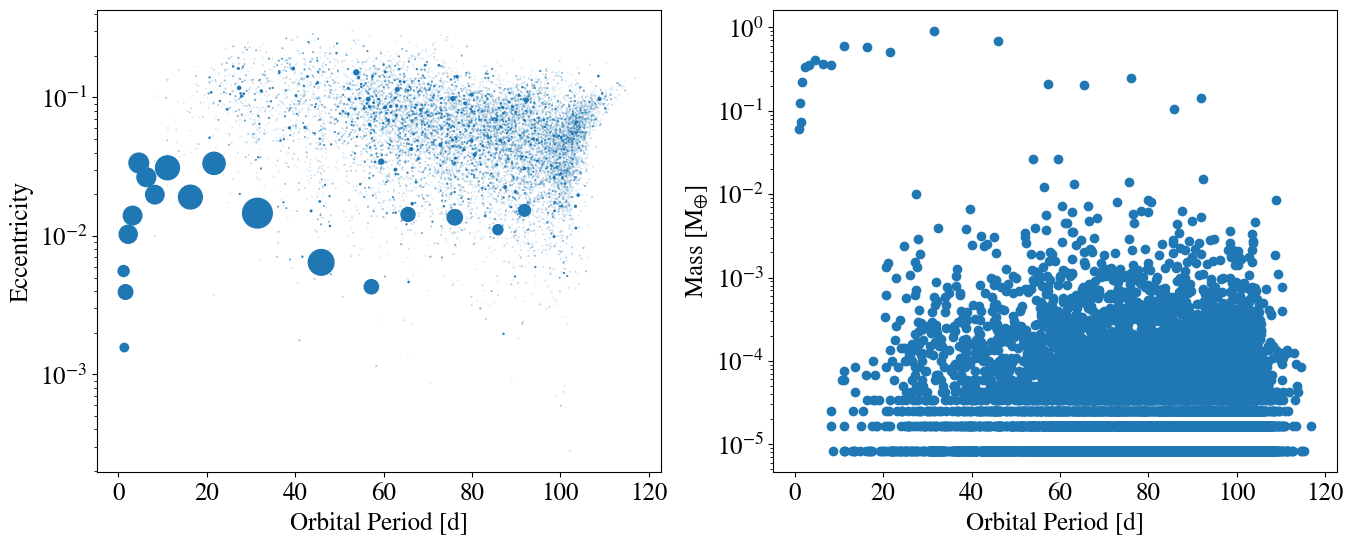
\includegraphics[width=\textwidth]{figures/stip/changa_ics.png}
    \caption{The period-eccentricity (left) and period-mass (right) distribution of a planetesimal growth simulation run to completion with {\sc ChaNGa}. A transition between non-oligarchic and oligarchic growth is visible around 40-60 days and is characterized by a change in the amount of residual planetesimals, along with a change in the masses of the protoplanets. The positions, velocities and masses of these bodies are then used as initial conditions for a {\sc genga} simulation, which is run until a fully-formed set of terrestrial planets are constructed.\label{fig:changa_ics}}
\end{center}
\end{figure*}

\subsection{Typical Planet Formation ICs: Isolation Mass Embryos}

We also construct a set of initial conditions to match a more typical scenario for an N-body simulation of terrestrial planet formation. Here, protoplanets throughout the disk are already fully formed and roughly evenly spaced. Although not as realistic, this type of setup is much simpler to construct and requires far fewer self-interacting bodies, which is a common point of trouble for most planet  formation simulations.

As with the planetesimal disk, the protoplanets are placed on orbits between 1 and 100 days in orbital period, and the disk is constructed to contain the same amount of total mass (X earth masses). To place protoplanets, we begin at the outer disk edge and calculate the local isolation mass \cite{kokubo02}

\begin{equation}\label{eq:iso}
	M_{iso} = \left[ \frac{\left( 2 \pi a^2 \Sigma \tilde{b} \right)^3}{3 M_{*}} \right]^{1/2},
\end{equation}

\noindent where a is the current semimajor axis, $\Sigma$ is the local solid surface density (using $\delta = 1.5$) and $\tilde{b}$ is the local feeding zone size (in units of the Hill radius). Starting at the outer disk edge, protoplanets are place one-by-one and $\tilde{b}$ is then randomly chosen to be between 5 and 10. The current semimajor axis is then decremented by $\tilde{b}$, the local isolation mass is recalculated and another protoplanet is placed. This process repeats until the inner disk edge is reached.

The eccentricities and inclinations are randomly drawn from a uniform distribution $\in \left[ 0, 0.01 \right]$ and the longitude of periastron, longitude of ascending node and mean anomaly are randomly drawn from a uniform distribution $\in \left[ 0, 2 \pi \right]$. In total, 5 sets of initial conditions using different random number seeds are constructed and integrated for 1 Myr.

\section{Results} \label{sec:results}

\subsection{In-Situ Formation Starting from Planetesimals}

One of the motivating questions for this work is whether a fully in-situ formation model leaves any distinct imprints of the orbital architecture of the resulting planets. By stitching together the snapshots from both phases of the simulation and reconciling the particle IDs, we can construct and examine the full history of the collision and phase space evolution for the entire ensemble of particles. In all cases, the planetesimal disks start out with just under $10^{6}$ particles and eventually consolidate into 5-10 super Earths, with around $10^{4}$ particles being ejected during the giant impact phase.

In figure \ref{fig:full_coll_evo}, we show the evolution of the orbits and the timing of collisions between bodies in the standard MMSN profile ($\delta = 1.5$) simulations. The gray curves show the orbital periods of the last 100 bodies to exist in each iteration of the simulation. The green curves indicate bodies which survived until the end of the simulation, where the line width denotes relative mass. Overlaid on top of the evolution curves are triangle markers, whose position on the plots indicates the instantaneous orbital period and timing of each collision event. The size of the markers indicates the relative mass of the body participating in the collision. In all cases, the secondary (less massive) body's state is used to determine the size and placement of the marker. Finally, the vertical blue line indicates the time at which the simulation state was transferred from {\sc ChaNGa} to {\sc genga}.

In all cases, its apparent that the bodies in the non-oligarchic growth region (P $<$ 40 d) behave in a qualitatively different way during the giant impact phase. Rather than scattering events and instability propagating from inside-out in the disk, the opposite appears to be true. The inner disk remains in a meta-stable state while the outer bodies undergo scattering and giant collisions first. We postulate that this is due to the presence of a residual planetesimal population in the outer disk, which acts to facilitate a gradual inward `random walk' of the protoplanets until they have a close encounter with another large body. This effect was also seen in \cite{murrayclay06} when modeling the outer solar system, and was even seen to facilitate capture of the planets into resonance. This effect was found to be largely resolution dependent and resonance capture was only possible with a sufficiently fine-grained planetesimal disk. In any case, we attribute the much more static state of the inner disk to the lack of residual planetesimals in this region.

\begin{figure*}
\begin{center}
    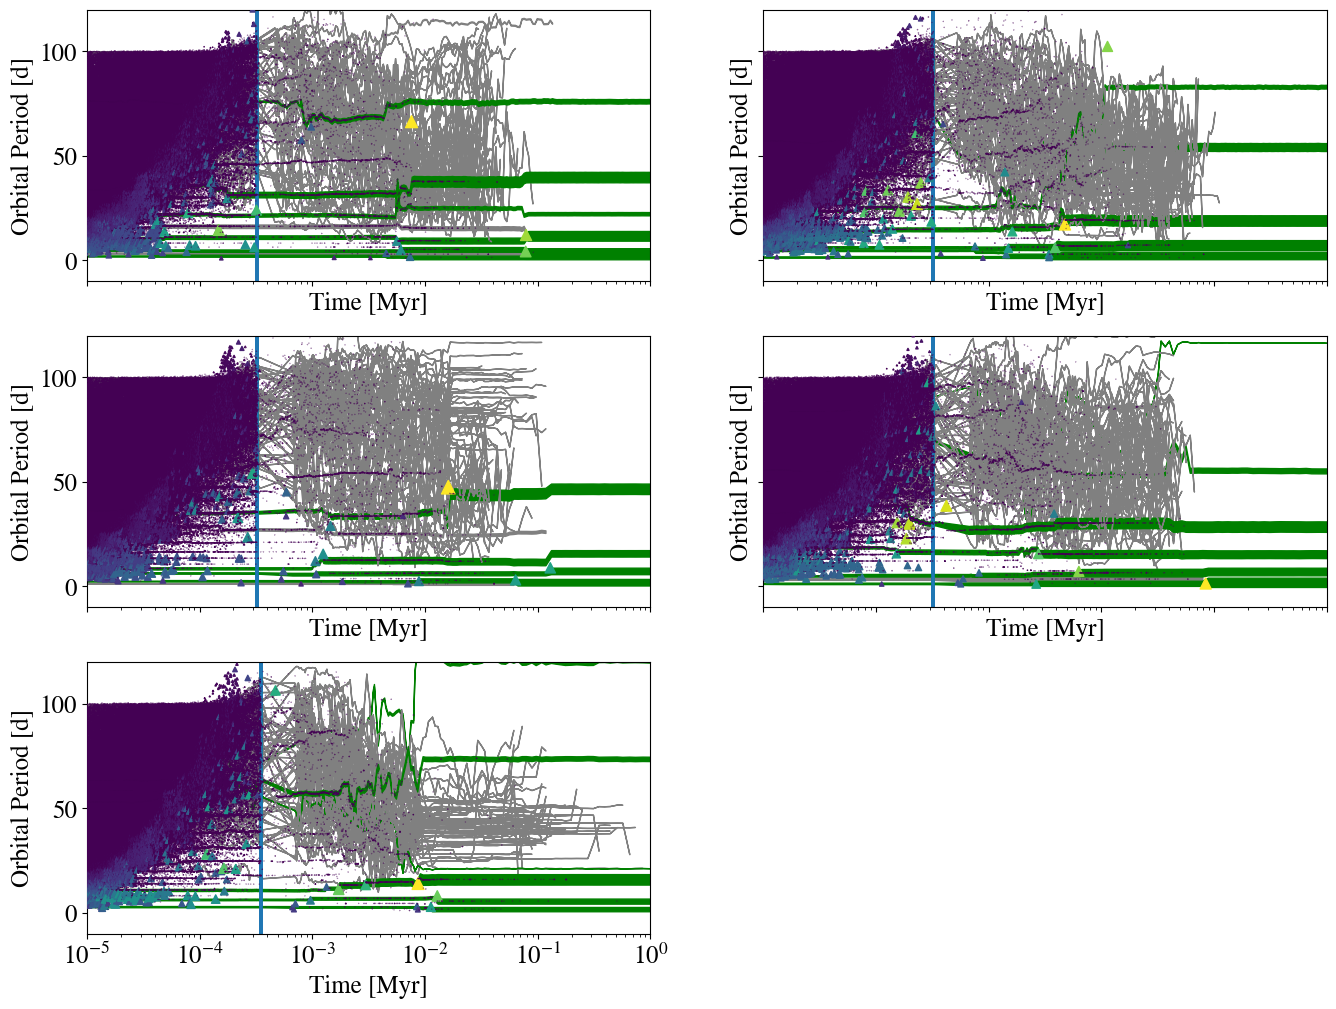
\includegraphics[width=\textwidth]{figures/stip/full_coll_evo.png}
    \caption{The evolution of the orbits of some of the last surviving bodies in the $\delta = 1.5$ simulations. Collisions are indicated with colored triangles, where the size and color denotes the relative mass of the body that was consumed in the merger. Green curves indicate bodies which survived through the end of the simulation and the line width indicates their relative mass. The vertical blue line marks the time at which the {\sc ChaNGA} snapshots were passed to {\sc genga}.\label{fig:full_coll_evo}}
\end{center}
\end{figure*}

Next, we examine the final configurations of the simulated planetary systems. In figure \ref{fig:per_mass_full}, we show the final period-mass distributions for all three choices of the initial surface density profile. Planets in the same system are connected by a solid line and each choice of random number seed for the initial conditions is shown as a different color. In most cases, the planet mass increases with orbital period and then turns over at some intermediate value. The turnover distance appears to be inversely proportional to the power law slope of the initial planetesimal disk $\delta$. In addition, there is some significant scatter in the final planetary architectures formed which is particularly prevalent for smaller values of $\delta$. This is driven by the role that chaos plays during the giant impact phase. In section \ref{sec:neuralICs}, we will revisit this aspect of the simulations and use a neural network to generate a much larger set of late-stage initial conditions which can then be evolved with {\sc genga}.

\begin{figure*}
\begin{center}
    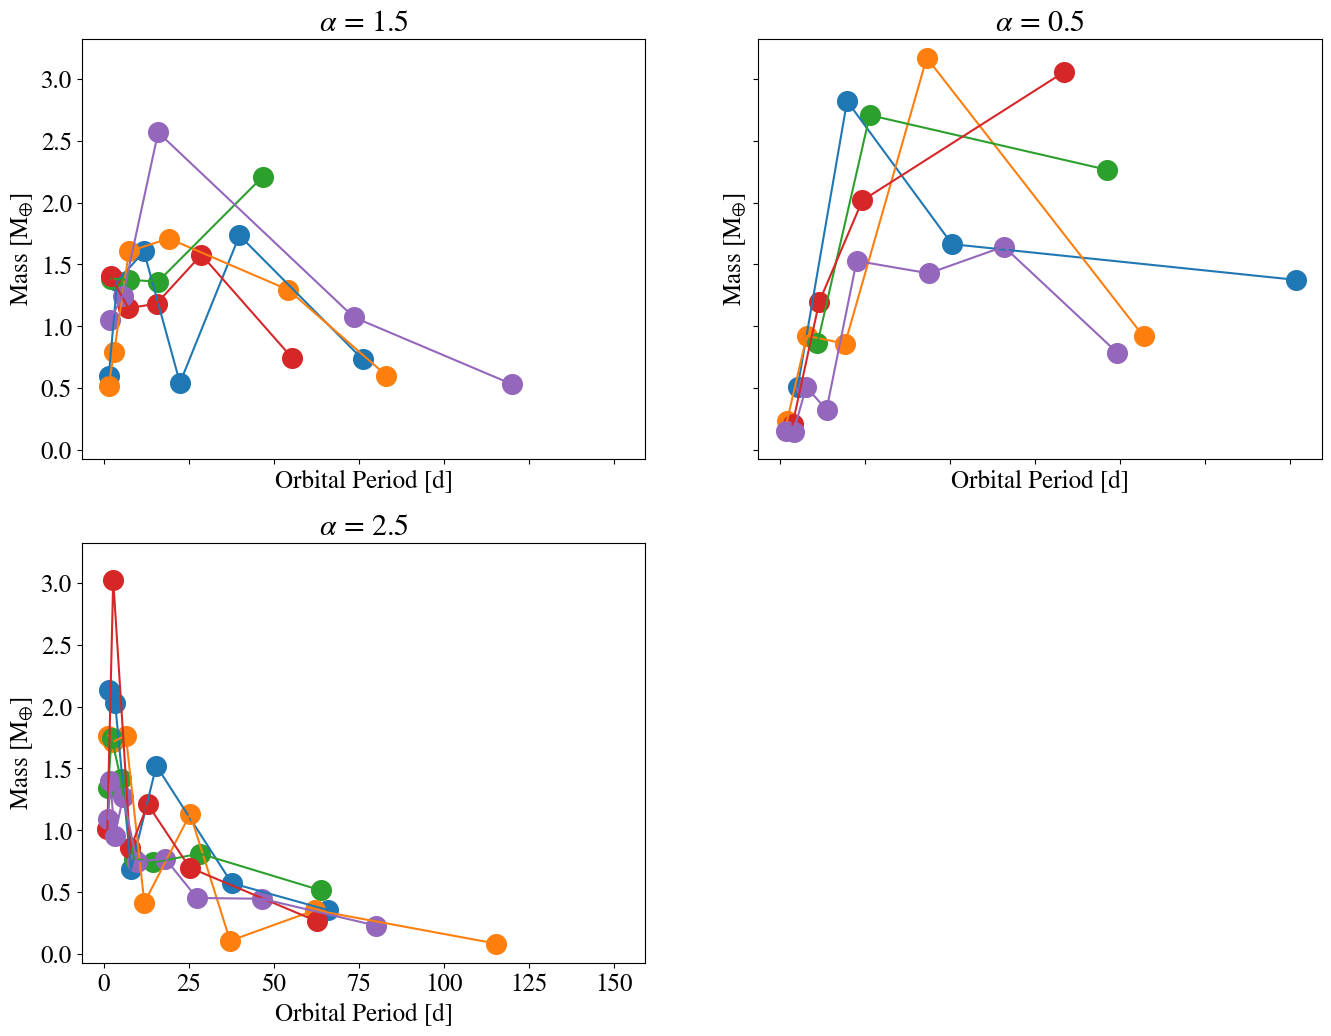
\includegraphics[width=\textwidth]{figures/stip/per_mass_full.png}
    \caption{Final period-mass configurations for the planets formed in all fifteen simulations. Each panel contains a set of simulations using a different mass surface density profile. Points connected by lines represent planets from the same simulation snapshot. Each color represents a set of initial conditions constructed from a different random number seed.\label{fig:per_mass_full}}
\end{center}
\end{figure*}

Having directly tracked every collision starting from the planetesimal phase allows us to make composition predictions for the resulting planets. To do so, we construct a collision tree for each planet in the final simulation snapshots, where the root node is the planet itself and the leaf nodes correspond to the initial mass planetesimals that went into its assembly. We place a snowline partway through the disk and for each planet, calculate the fraction of consumed planetesimals which originated from beyond the snowline location. Due to the fact that the inflated collision cross sections used during the planetesimal accretion phase alter the location of the accretion mode boundary in the disk (see Wallace + Quinn 2023), along with the fact that the snow line locations should be expected to vary widely over the course of the central star's pre-main sequence evolution \cite{baraffe15}, we choose to simply place a static snowline at 50 days in orbital period.

Figure \ref{fig:snowline} shows the expected wet/dry compositions of the planetary systems formed in the $\delta = 1.5$ simulations. Each row of points on the y-axis corresponds to a separate iteration of the simulation and the point sizes indicate relative masses. The blue shading represents the total mass fraction of accreted planetesimals that originated from beyond the snowline, which is indicated by a vertical line. In all cases, we see that water-rich material is able to be incorporated into planets far interior to the snowline location. In one case, a significantly dry planet eventually ends up well beyond the snowline.

As our model is purely in-situ and does not incorporate any significant dissipative forces from the gas disk, one would not expect any resonant chains to form. However, some recent work \cite{izidoro17, raymond18} has shown that super-Earths in resonant chain configurations can later destabilize. One would therefore wonder whether there is any distinguishable difference between a super-Earth system that had formed purely in-situ, and one that underwent convergent migration and was then destabilized. \cite{raymond18} found that the inward migration of wet embryos can actually concentrate and consolidate rocky material near the inner edge of the disk. This quality is also present in our in-situ systems. \cite{izidoro17}, however, found that only about 50 percent of resonant chains eventually go unstable, while 75 percent must do so to match observations. Given that our in-situ systems appear rather qualitatively similar to the convergent migration, followed by destabilization driven systems seen by \cite{raymond18}, it may be the case that disk-driven migration simply doesn't operate for some fraction of STIPs.

\begin{figure}
\begin{center}
    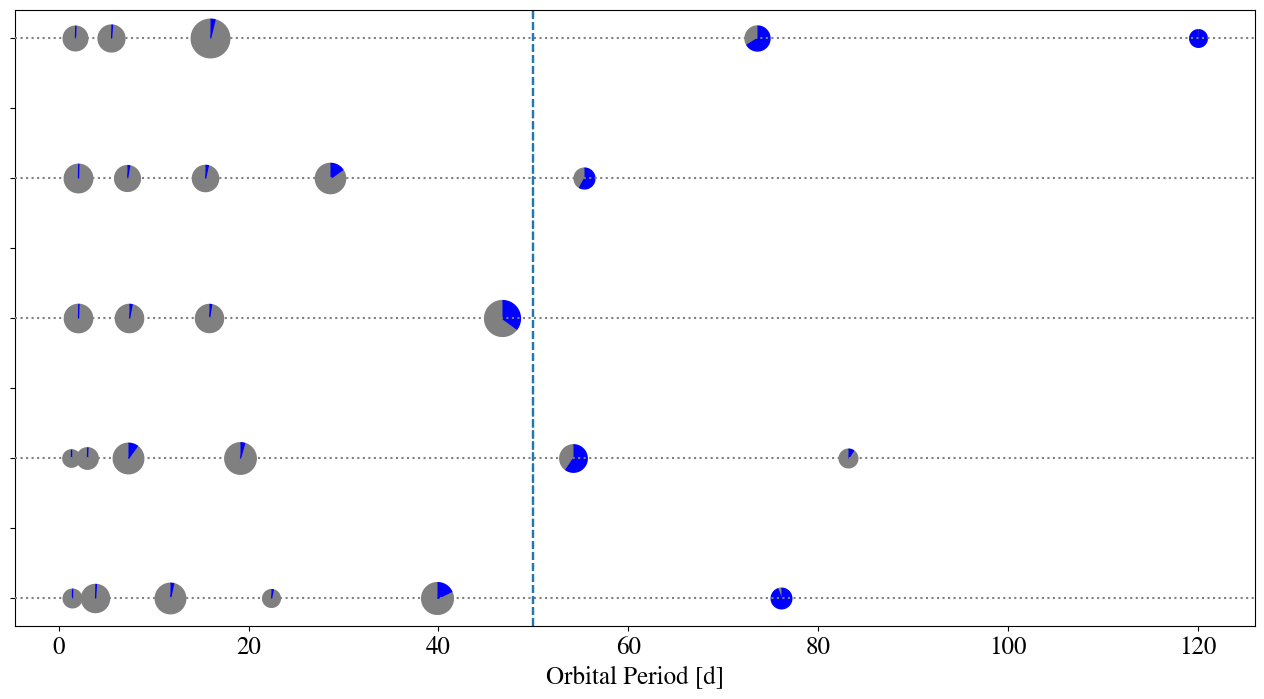
\includegraphics[width=0.5\textwidth]{figures/stip/snowline.png}
    \caption{Final compositions of planets from the five $\delta = 1.5$ simulations. Point sizes indicate relative mass and the pie fractions indicate the amount of wet/dry material incorporated into each planet. A snow line is placed at 50 days in orbital period and all planetesimals that originate from beyond this location are assumed to be wet.\label{fig:snowline}}
\end{center}
\end{figure}

\section{Comparison With Typical Planet Formation ICs} \label{sec:typicalICs}

The simulations presented in this work are not the first to investigate the outcome of an in-situ model on the formation of STIPs (see \cite{hansen12}). However, this work does self-consistently follow the terrestrial planet formation process from some of the smallest gravitationally bound objects, which is not the case for most planet formation N-body simulations. Typically, these types of simulations begin with either a set of equal-mass embryos placed in a wide annulus \cite{obrien06}, or a set of regularly spaced embryos that follow the local isolation mass of the disk (e.g. \cite{raymond05, raymond06, hansen12}). There are two implicit assumptions made in these models: 1. The embryo formation process behaves in a self-similar manner everywhere in the disk. 2. The embryo formation process has fully completed everywhere in the disk before the giant impact phase initiates. Assumption number two is generally valid for the inner solar system, as the planetesimal accretion timescale is much shorter than the instability timescale which gives rise to the giant impact phase \cite{chambers96}. However, assumption number one is not physically motivated.

As we showed in (Wallace + Quinn 2023), the oligarchic growth process, which gives rise to planetary embryos, should only be expected to operate down to $\sim$ 5 days in orbital period. Furthermore, the late-stage instability that initiates collisions between protoplanets is a nonlinear process and there have yet to be any investigations of how it behaves at short period. Both of these concerns are naturally addressed in the simulations we present in this chapter. Except for the fact that the non-oligarchic accretion boundary has been moved out by a factor of a few in orbital period due to the inflation of the collision cross sections during the planetesimal growth phase, the state of the protoplanets at the beginning of the {\sc genga} simulations is free from any simplifying assumptions. To understand the influence that these simplifications made in typical N-body simulations of planet formation have on the final architectures of the systems, we compare our $\delta = 1.5$ simulations with a set of late-stage simulations which begin with fully-formed, isolation mass embryos in a disk with an identical mass profile.

\begin{figure*}
\begin{center}
    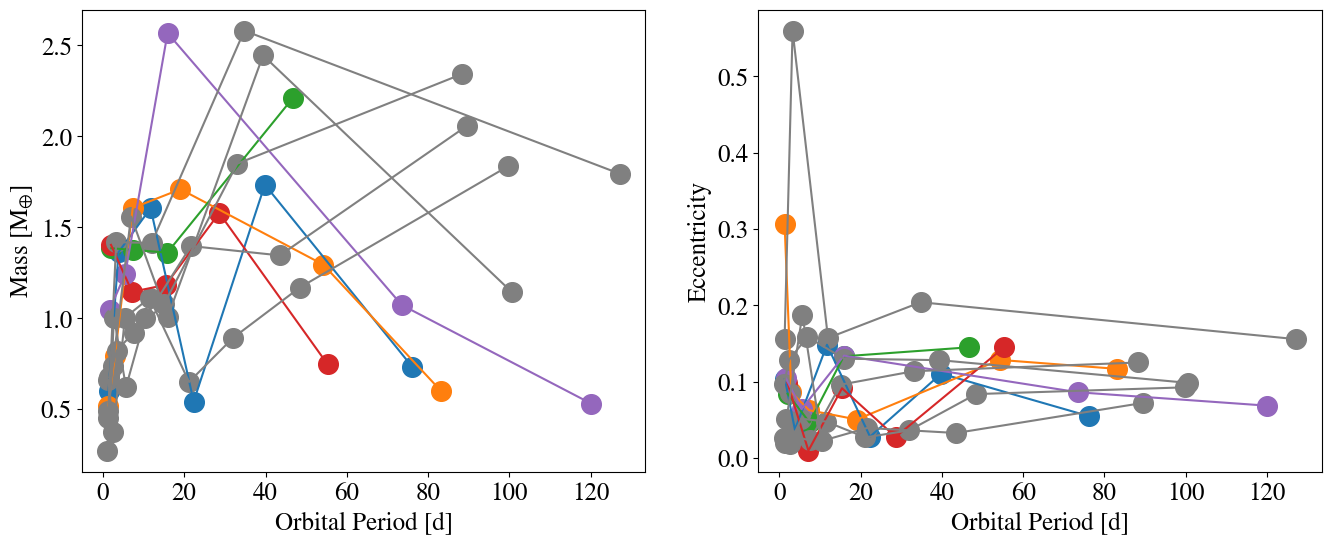
\includegraphics[width=\textwidth]{figures/stip/per_mass_ecc_iso_comp.png}
    \caption{The period-mass (left) and period-eccentricity (right) distributions of the simulations starting from planetesimals (colored points) and isolation mass embryos (gray points). Each planetary system is connected by a series of lines.\label{fig:per_mass_ecc_iso_comp}}
\end{center}
\end{figure*}

In figure \ref{fig:per_mass_ecc_iso_comp}, we compare the period-mass and period-eccentricity distributions of the planetary systems formed starting from planetesimals and starting from isolation mass embryos (shown in gray). Qualitatively, the eccentricity distributions are remarkably similar between the two sets of initial conditions, despite the fact that the protoplanet eccentricites at the end of the planetesimal accretion simulations start off nearly an order of magnitude smaller than the isolation mass embryos. The period-mass distributions, however, show some noticeable differences.

Overall, the isolation mass embryo simulations tend to form larger planets. There are twice as many $> 2 M_{\odot}$ planets using the fully formed isolation mass set of initial conditions. In addition, the mass in these simulations tends to be less radially concentrated, with every single set of initial conditions producing a super-Earth beyond 80 days in orbital period. In contrast, two of the simulations starting from planetesimals produce a truncated set of planets that do not extend beyond 60 days. Most noticeably, the isolation mass embryo simulations produce a wider variety of masses and eccentricities between sets of initial conditions. This highlights the more influential role that stochasticity plays in these simulations. One possibility for this difference comes from the fact that the isolation mass embryo simulations do not contain any planetesimals, and the gravitational kicks between embryos do not get damped out. A second possibility comes from the way in which the instability which gives rise to the giant impact phase propagates through the disk in each case. For the simulations starting from planetesimals, there is a qualitative difference between the inner and outer disk, and the onset of chaos may occur in a different fashion.

To test this second hypothesis, we examine the timing and location of collisions in the disk for each set of simulations. In figure \ref{fig:full_coll_iso_comp}, we show ensemble of collisions recorded in all five versions of the simulations starting from planetesimals (blue points) and isolation mass embryos (orange points). The point sizes indicate the relative masses of bodies consumed in the merger events. The orbital period of each collision is calculated using the phase space state of the consumed body at the moment of impact. For the isolation mass simulations, the collision times are offset by the integration time of the {\sc ChaNGa} simulations because there is no prior planetesimal accretion phase.

During the giant impact phase, there is a clear qualitative difference in the location and timing of protoplanet collisions between the two sets of simulations. For the isolation mass embryo simulations, giant impacts begin almost immediately at the inner edge of the disk and propagate outward over a timescale of $\sim 10^{4}$ years. For the simulations starting from planetesimals, the commencement of giant impacts is nearly simultaneous everywhere in the disk. Additionally, this phase seems to be much longer-lived, particularly beyond about 20 days in orbital period.

The near-instantaneous initiation of the giant impact phase in the simulations starting from planetesimals is a possible explanation as to why the variation in the final masses and eccentricites of the resulting planets is smaller. In contrast to the isolation mass simulations, giant impacts occur nearly everywhere in the disk simultaneously, which acts to damp eccentricities and reduces the distance over which protoplanets can communicate. A smaller interaction distance therefore reduces the possible outcomes of the giant impact phase and produces a smaller scatter in the final masses and eccentricities. Because collisions tend to happen at perihelion \cite{levison03}, protoplanets that are simultaneously excited in the outer disk tend to collide in the inner disk, which explains why there are so few planets end up in the outer disk for this set of simulations. The isolation mass embryos, on the other hand, interact with the rest of the disk in an inside-out fashion. This dynamically excited outward-propagating boundary has the opportunity to interact the entire outer disk, which is still an a non-excited state. Between different iterations of the simulation, scattering events happen at different points along an excited protoplanets orbit, which widens the possibilities for the final orbital configurations of the resulting planets. (Talk about role of planetesimals as well?)

\begin{figure*}
\begin{center}
    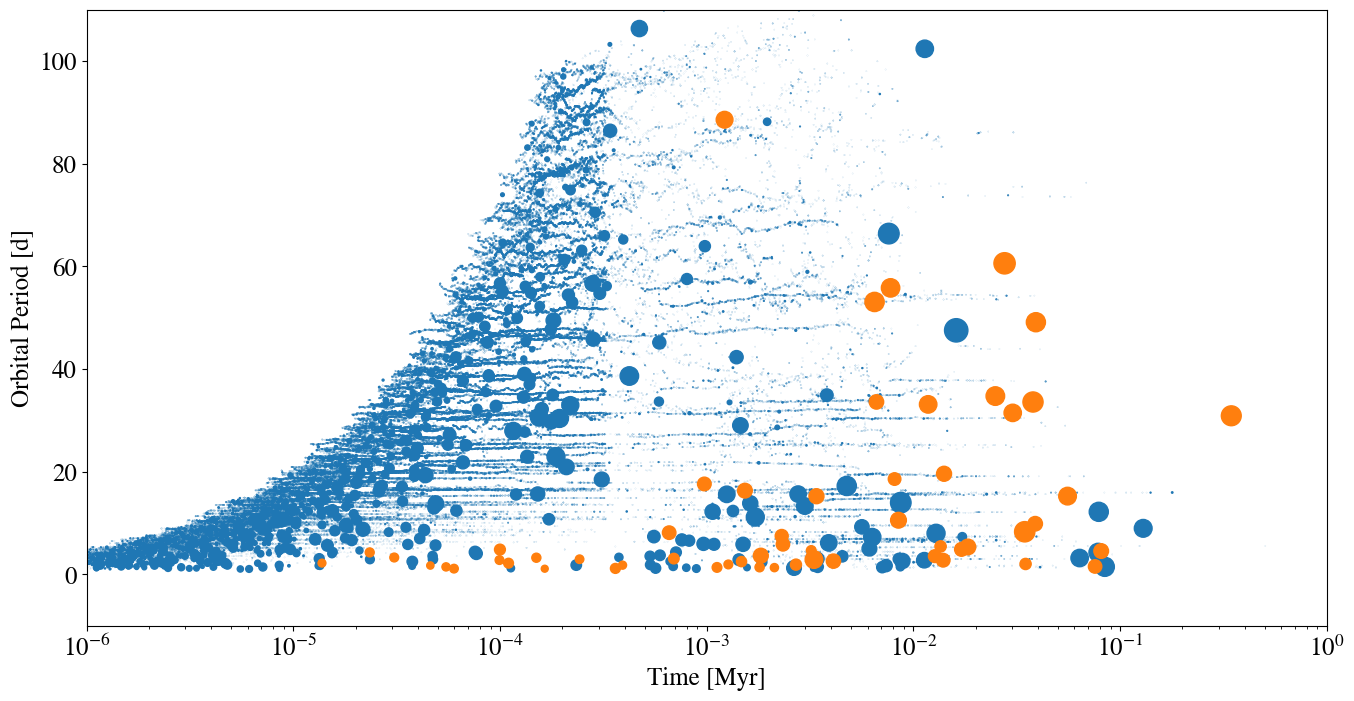
\includegraphics[width=\textwidth]{figures/stip/full_coll_iso_comp.png}
    \caption{Figure caption goes here.\label{fig:full_coll_iso_comp}}
\end{center}
\end{figure*}

Lastly, we examine the relative collision velocities of growing protoplanets during the giant impact phase. \cite{volk15} proposed that the lack of short-period planets in the solar system is due to an earlier phase of violent instability in the inner disk which destroyed any such worlds. Given the sudden onset of instability in our simulations starting from planetsimals, one might wonder whether some of the later collisions should be destructive. Because all collisions result in perfect mergers in our simulations, this effect is not self-consistently captured, but we can examine the collision statistics afterwards to determine which planets might have undergone earlier destruction.

In figure \ref{fig:impact_iso_comp}, we show the timing and speed of collisions between bodies larger than 0.01 $M_{\odot}$ in each set of simulations. The gray points denote collisions from the isolation mass simulations, while the colored points indicate collisions from the simulations started from planetesimals. The collision speeds on the y-axis are shown in units of the mutual escape velocity of the colliding particles. For super-Earth and smaller sized bodies, $v_{coll}/v_{esc} > 2$ tends to produce destructive collisions \cite{marcus09} and so we have marked this region of the figure with a horizontal dashed line. Solid lines connecting points indicate subsequent collisions between the same body.

With the exception of a single high-speed collision around $T = 20,000$ yr, (and another collision right on the destruction/accretion boundary) none of the collisions from the isolation mass simulations can be roughly categorized as destructive. In contrast, every simulation starting from planetesimals eventually produces at least one destructive collision. In three of these cases, multi-collision excitation eventually leads to a destructive encounter, which is the same mechanism seen by \cite{volk15}.

In figure \ref{fig:impact_iso_comp}, we show the final orbital architectures of all ten simulations. Here, point sizes indicate relative mass and the simulations starting from planetesimals are colored blue, while the isolation mass embryo simulations are colored gray. Planets that underwent a destructive collision during their giant impact phase are marked with a red X. For the simulations starting from planetesimals, the destructive collisions all involve the planets at the innermost edge of the disk. This is only the case for one of the isolation mass embryo simulations. 

\begin{figure}
\begin{center}
    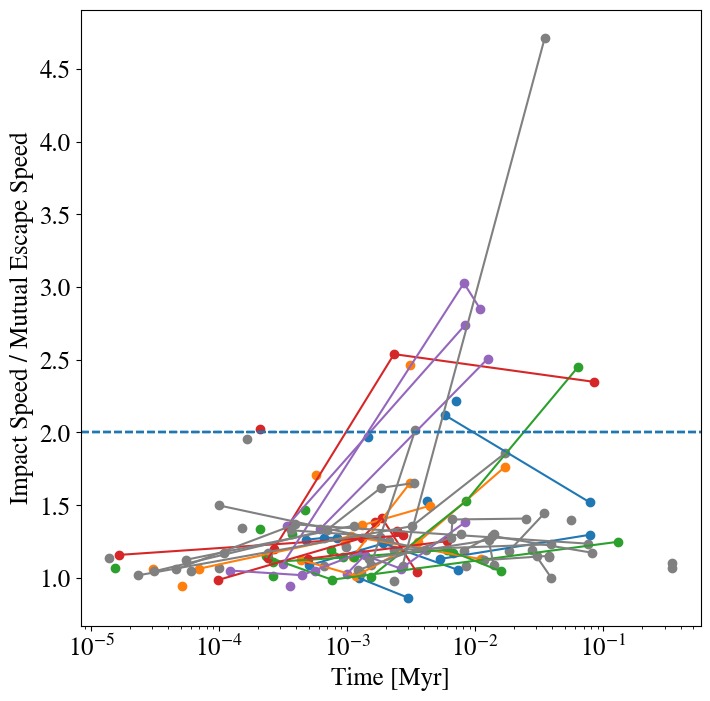
\includegraphics[width=0.5\textwidth]{figures/stip/impact_iso_comp.png}
    \caption{Figure caption goes here.\label{fig:impact_iso_comp}}
\end{center}
\end{figure}

Although $v_{coll}/v_{esc} > 2$ are expected to be at least partially destructive \cite{marcus09}, it is not immediately clear whether the debris should be expected to re-accrete onto other bodies or be entirely removed from the system. For small grains (1-10 microns), dust blow out can entirely eject material from the system on timescales much shorter than re-accretion. Larger grains (cm-sized) can be removed by PR drag on $10^{5}$ yr timescales. This is particularly efficient if the timescale for collisional grinding of debris is fast \cite{melis12}. For planetesimal-sized objects (100 km), gravitational scattering can eventually eject material. This was the eventual fate of most remaining planetesimals at the end of the {\sc ChaNGa} simulations.

Another caveat is that the integration time we use (1 Myr) is only a small fraction of the age of most STIPs \cite{silvaaguirre15} and our results should only be interpreted as applicable to expected behavior during the gaseous disk phase of the planet formation process. The solar system is thought to be in a state of constant metastability, having an instability timescales that matches its current age \cite{laskar96}. The same is likely true for many exoplanetary systems as well (see \cite{deck12, lissauer12, lissauer13}). In addition, the small sample size of our 5 simulations in each configuration is unlikely to have captured the full extent of the effects of dynamical chaos during the giant impact phase. To address this second point, we train a neural network to produce a much larger set of qualitatively similar, but numerically distinct initial conditions to pass to {\sc genga}, which we describe in detail in the next section.

\begin{figure}
\begin{center}
    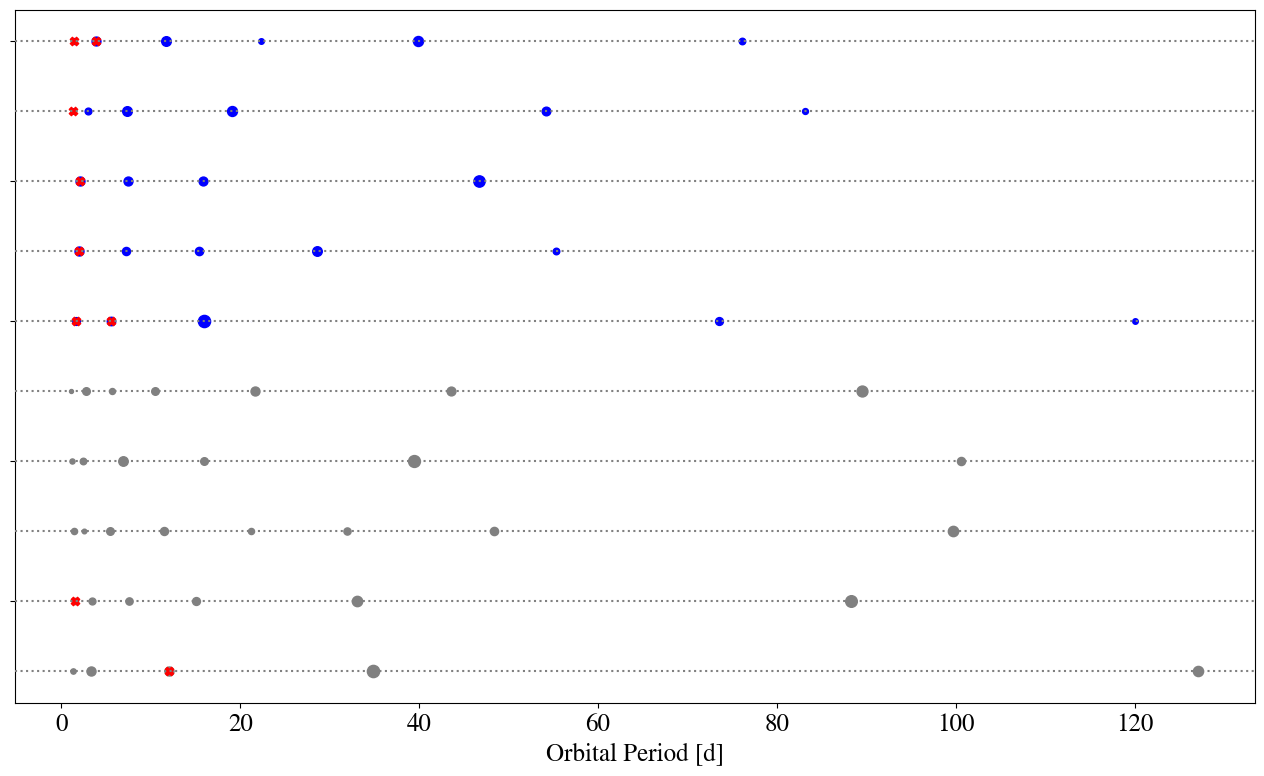
\includegraphics[width=0.5\textwidth]{figures/stip/architectures_iso_comp.png}
    \caption{Figure caption goes here.\label{fig:architectures_iso_comp}}
\end{center}
\end{figure}

\section{Training a Neural Network to Synthesize ICs} \label{sec:neuralICs}

To fully capture the role that stochasticity plays during the protoplanet assembly phase, a much larger set of simulations is required. As we have shown in the previous section, using a typical arrangements of isolation mass embryos to set up the giant impact phase does not seem to be sufficient. Each of the planetesimal accretion simulations run with {\sc ChaNGa}, however, require about 80,000 CPU hours. Passing each of these simulations to {\sc genga} and integrating to 1 Myr requires another 200 or so GPU hours. The large particle count, in addition to the fact that different parts of the disk evolve semi-independently of each other, means that stochasticity does not play an important role during the planetesimal accretion phase and a small number of simulations is sufficient to capture the outcome of the embryo formation process. When trying to capture the full breadth of planetary architectures possible with our in situ model, it is most useful to focus our computational resources on the {\sc genga} simulations. Doing so requires a much larger set of late-stage initial conditions.

Although there is very little qualitative variation between the {\sc ChaNGa} simulations run in each initial disk configuration, slight differences in the masses, positions and velocities of the embryos and planetesimals lead to significantly different planetary systems, due to the chaotic nature of the giant impact phase. To generate numerically distinct late-stage initial conditions requires an underlying model for orbital distributions of the planetesimals and embryos. Given the presence of the accretion boundary at short period, an analytic model is likely insufficient. Instead, we use the existing simulation snapshots to construct posterior distributions for the particles, and then randomly draw from these distributions to generate more initial conditions.

\subsection{Training a Generative Adversarial Network}

We use an unsupervised machine learning technique known as a Generative Adversarial Network (GAN). A GAN is a deep learning method \cite{goodfellow14}, that uses two separate neural networks, a generator and a discriminator, to train itself to produce an infinite collection of qualitatively similar datasets based on some input training data.

GANs are most well-known for use in synthetic image generation, and first gained traction in the astronomy community when they were used to enhance \cite{schawinski17} and even produce entirely new galaxy images \cite{dia20}. GANs have also recently been applied to N-body simulations to do things such as map large-scale gas and temperature distributions \cite{troster19} and generate mock galaxy catalogs \cite{jagvaral22}. In the planetary domain, GANs have been used for exoplanet atmosphere retrieval \cite{zingales18} and even to supplement transit detection models \cite{dvash22}.

In a traditional GAN, the discriminator and generator are pitted against each other. A noise vector is fed to the generator which is used to produce a synthetic dataset. The synthetic data is then fed to the discriminator, alongside the original training data. The discriminator then determines whether the two datasets are distinguishable. In the case that the synthetic data is classified as `fake', a loss function is calculated and the result is used in a backward pass through both neural networks to update the weights. Over many iterations, the generator improves its ability to produce authentic-looking synthetic data and the discriminator gets better at distinguishing between real and fake data. Once the discriminator reaches a point where roughly 50 percent of the synthetic data is classified as fake, the algorithm reaches an equilibrium and the generator is considered to be fully trained.

To construct a generator, we use the {\sc CTGAN} \cite{xu19} package to train a neural network on our planetesimal accretion simulation results. Traditional GANs are notoriously sensitive to issues such as non-convergence and mode collapse, both of which prevent the generator from ever being able to produce sufficiently varied and useful results. To combat these issues, {\sc CTGAN} models are trained using a WGAN loss function with a gradient penalty \cite{gulrajani17}. Updates to the generator and discriminator between iterations are done using an Adam optimizer \cite{kingma14}, which is a stochastic gradient descent algorithm. Both neural networks are updated using a learning rate of $2 \times 10^{-4}$.

One challenge when working with unsupervised machine learning techniques is determining the best way to format and represent the training data. In the case of the our planetesimal accretion simulations, the residual planetesimals greatly outnumber the protoplanets, which causes the neural networks to place much more emphasis on the planetesimal distribution. One solution to this problem is to modify the loss function to give more weight to the protoplanets. {\sc CTGAN}, however, does not provide a way to modify the loss functions, and we found that this approach did not work well in our own experiments when constructing a toy model. A simpler solution is to give every particle in the data set a mass of $m_{0}$ and then duplicate points based on their original mass. In addition to expanding the size of the training data set by a factor of nearly 100, this causes the GAN algorithm to fall into a perpetual state of non-convergence.

An even simpler solution that works well with our simulation data is to simply split the dataset in two, with a mass cut that cleanly separates the protoplanets from the remaining planetesimals. To train our GAN, we concatenate all of the final $\delta = 1.5$ {\sc ChaNGa} snapshots into a single table and place a mass cut at 0.03 $M_{\oplus}$ to split the dataset into two parts. The state of the particles are passed to the deep learning algorithm in terms of orbital period, and logarithmic eccentricity, logarithmic inclination and logarithmic mass. To quantify the accretion histories of the particles, we also include the `smooth accretion fraction' (see Wallace + Quinn 2023) as a separate column in the training sets. Doing so naturally incorporates the effects of the oligarchic and non-oligarchic accretion modes into the data and substantially helps to tighten up the period-mass relation of the synthetic protoplanets.

\begin{figure*}
\begin{center}
    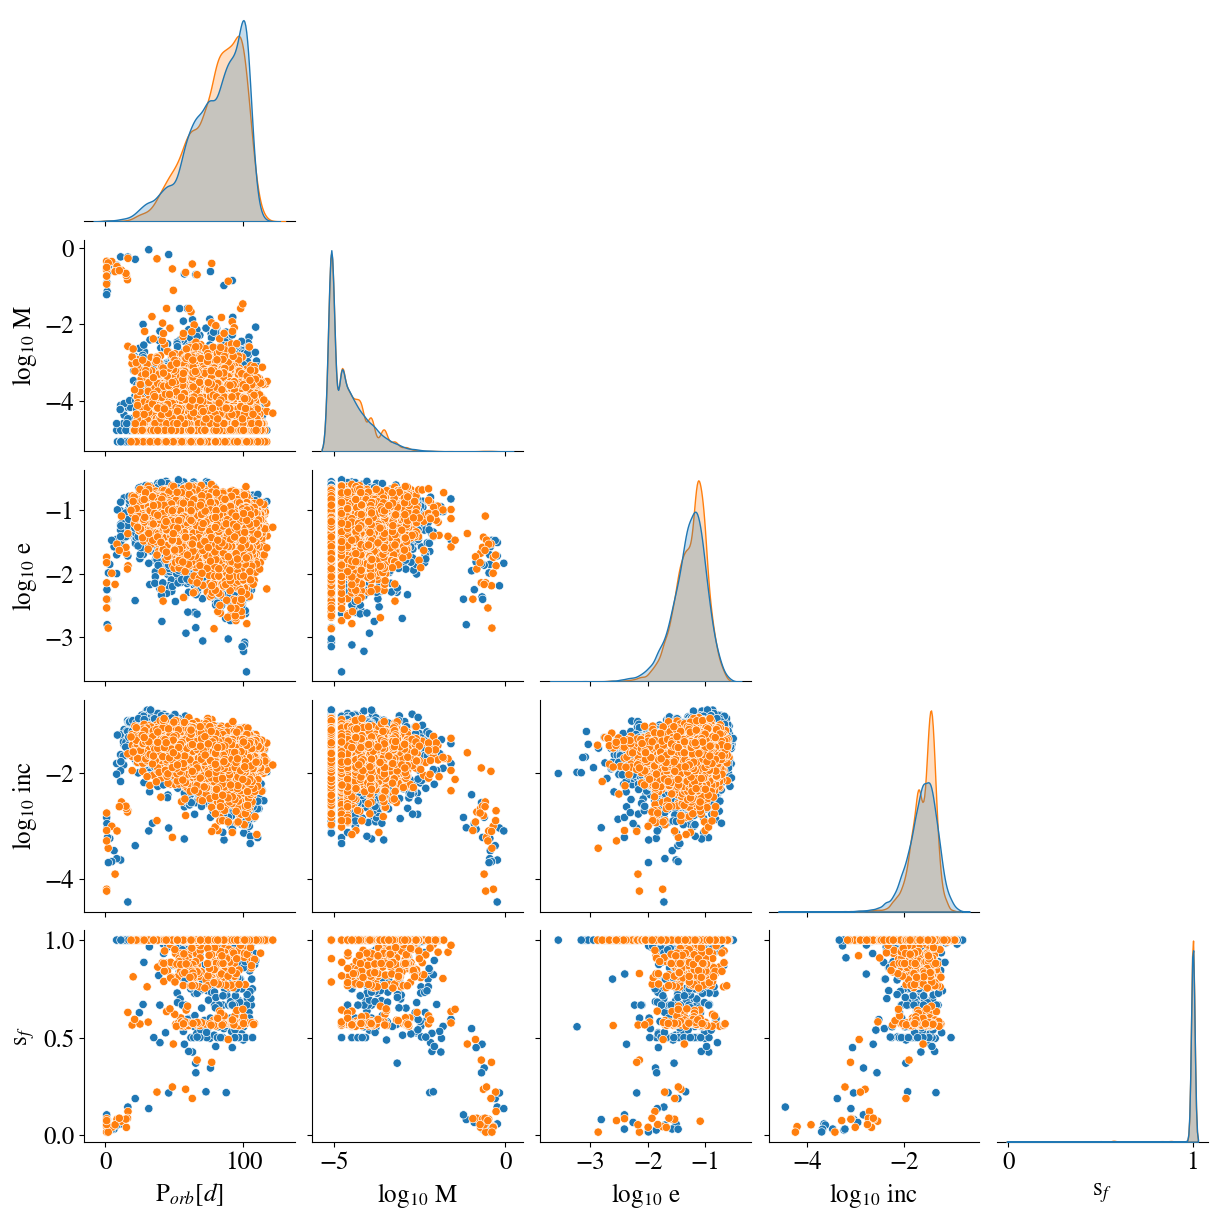
\includegraphics[width=\textwidth]{figures/stip/real_syn_corner.png}
    \caption{Figure caption goes here.\label{fig:real_syn_corner}}
\end{center}
\end{figure*}

In figure \ref{fig:real_syn_corner}, we show the correlations between the features used to train the GANs in the training (blue) and synthetic (orange) datasets after 5,000 epochs. The discretization of the masses (due to growth via perfect mergers) is clearly visible in the synthetic data, despite no enforcement of this property in the model. This characteristic of the mass data, however, appear to produce some additional small artificial peaks in the synthetic mass distribution at equal intervals in logarithmic space. To circumvent this issue, we also tried training the models using linear masses but it did not appear to reconcile the match between the real and synthetic mass distributions. Due to the weak, indirect role that planetesimals play during the giant impact phase, we chose to leave the synthetic mass distribution as-is.

To construct initial conditions from the synthetic data, particles are drawn one-by-one until the total mass exceeds the average disk mass of the full simulations. This is done separately for the planetesimal and embryo populations, and the total masses of each are matched accordingly. Out of the 100 sets of initial conditions we construct, the synthetic particle count matches the original particle count to within 5 percent, which is an encouraging sign that the generator is properly capturing the physical state of the disk.

Once particles are drawn using the five features that the neural networks were trained on, the longitude of periastron, longitude of ascending node and mean anomaly are randomly drawn $\in \left[0, 2 \pi \right)$ for each particle. The six orbital elements are then converted to cartesian coordinates and particle radii are calculated using the synthetic masses under the assumption that the bulk density is 3 g $cm^{-3}$. All 100 sets of initial conditions are passed to {\sc genga} and integrated to 1 Myr.

\begin{figure*}
\begin{center}
    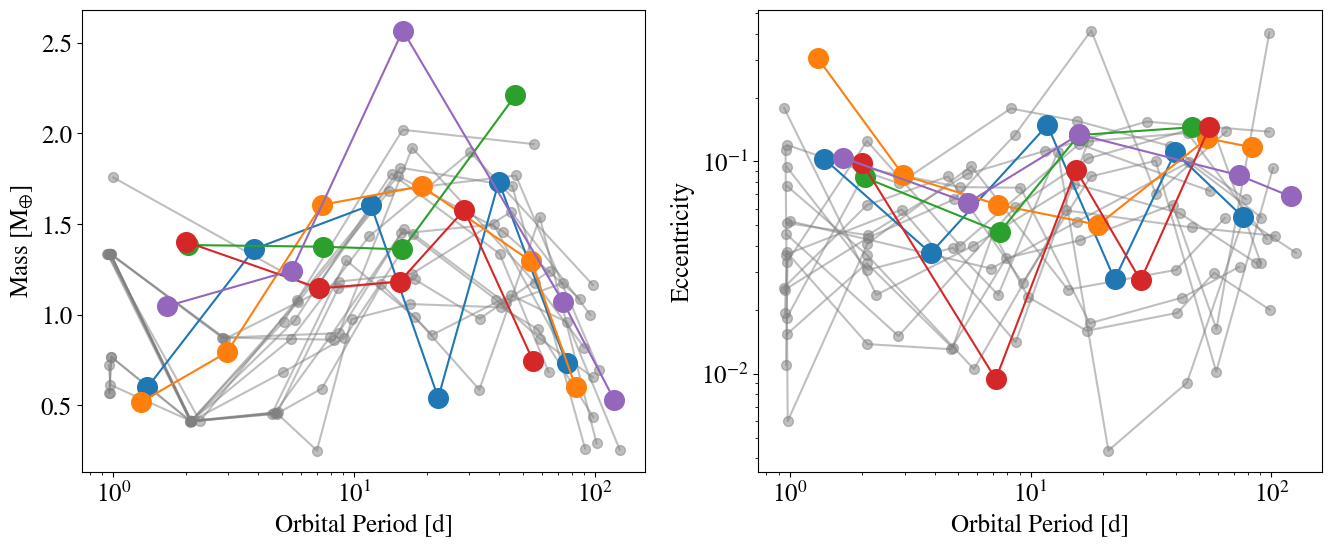
\includegraphics[width=\textwidth]{figures/stip/per_mass_ecc_syn_comp.png}
    \caption{Figure caption goes here.\label{fig:per_mass_ecc_syn_comp}}
\end{center}
\end{figure*}

In figure \ref{fig:per_mass_ecc_syn_comp}, we show the resulting period-mass and period-eccentricity distributions of the synthetic simulations (gray points) alongside the full simulations (colored points). Here, planets from the same system are connected by solid lines. The masses of the synthetic planets are quite similar to those in the full simulation, with the turnover in the period-mass relation occurring at roughly the same orbital period (20 days). The period-eccentricity distribution of both sets of simulations appears quite flat and both exhibit a similar mean eccentricity, which indicates that the giant impact phase plays out in a very similar way for the synthetic simulations. TODO: KS-test for real and synthetic mass, eccentricity distributions, the distributions are shown in figure 5.12.

\begin{figure*}
\begin{center}
    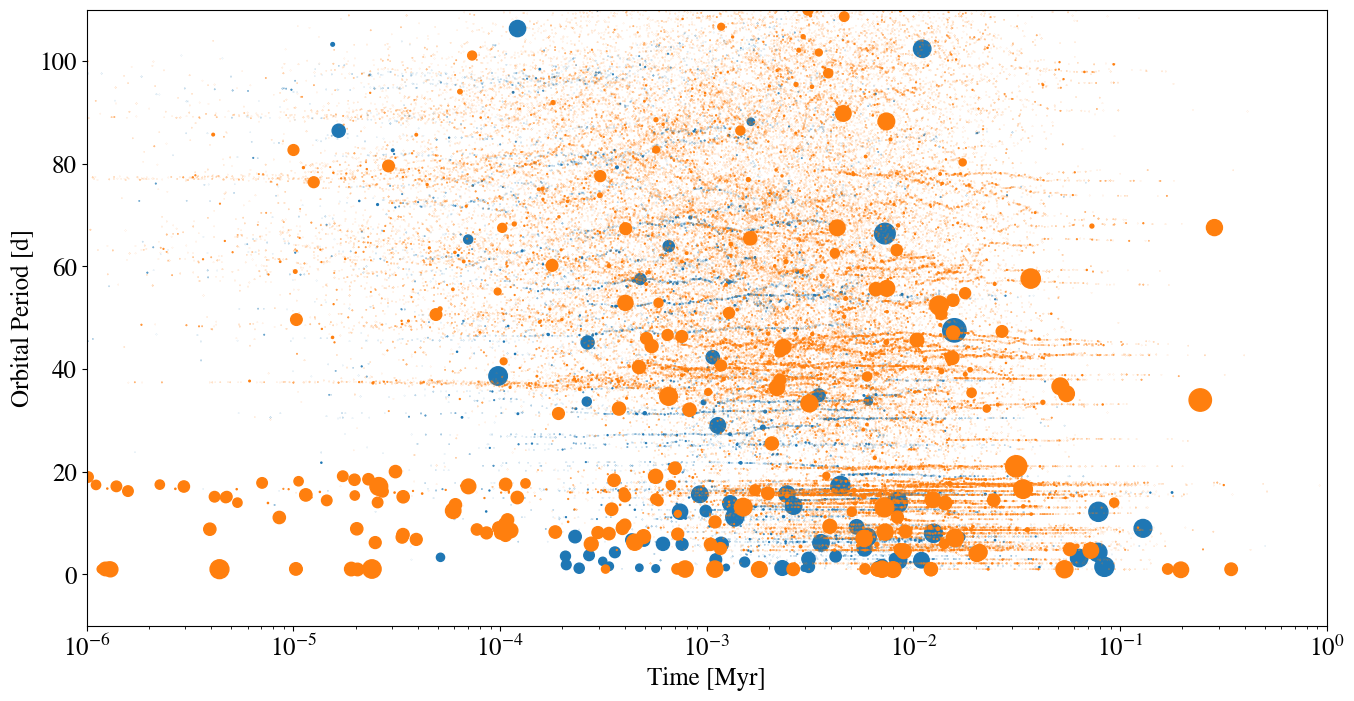
\includegraphics[width=\textwidth]{figures/stip/full_coll_syn_comp.png}
    \caption{Figure caption goes here.\label{fig:full_coll_syn_comp}}
\end{center}
\end{figure*}

Next, we examine the timing and location of collisions between the full and synthetic simulations. This is shown in figure \ref{fig:full_coll_syn_comp}, where point sizes indicate relative mass of the body consumed in a merger and the point location indicates the timing and orbital period (calculated from the instantaneous position and velocity at the moment of impact) of the body. In the inner disk, collisions take about 100 yr to get underway for the full simulations, while giant impacts begin almost immediately for the synthetic simulations. Despite the features of the training set and the synthetic dataset matching up well in this region of the disk, the generator does not appear to be producing embryos in a metastable configuration here. To date, most deep learning techniques require more than just particle phase space information at a single snapshot in time to make accurate stability classifications (see \cite{tamayo20, cranmer21}), so it is not unexpected that our neural network can't reproduce a metastable configuration of embryos.

With the exception of the inner 20 day orbital period region of the disk, giant impacts occur in a nearly instantaneous fashion for both the full and synthetic simulations, which is promising evidence that the synthetic data is still reproducing some of the same dynamical behavior as the training dataset. This also suggests that the early onset of giant impacts in the synthetic inner disk is not affecting the growth of planets elsewhere and is not a major concern. In addition, the resulting planetary masses in the inner disk are quite similar.

\begin{figure*}
\begin{center}
    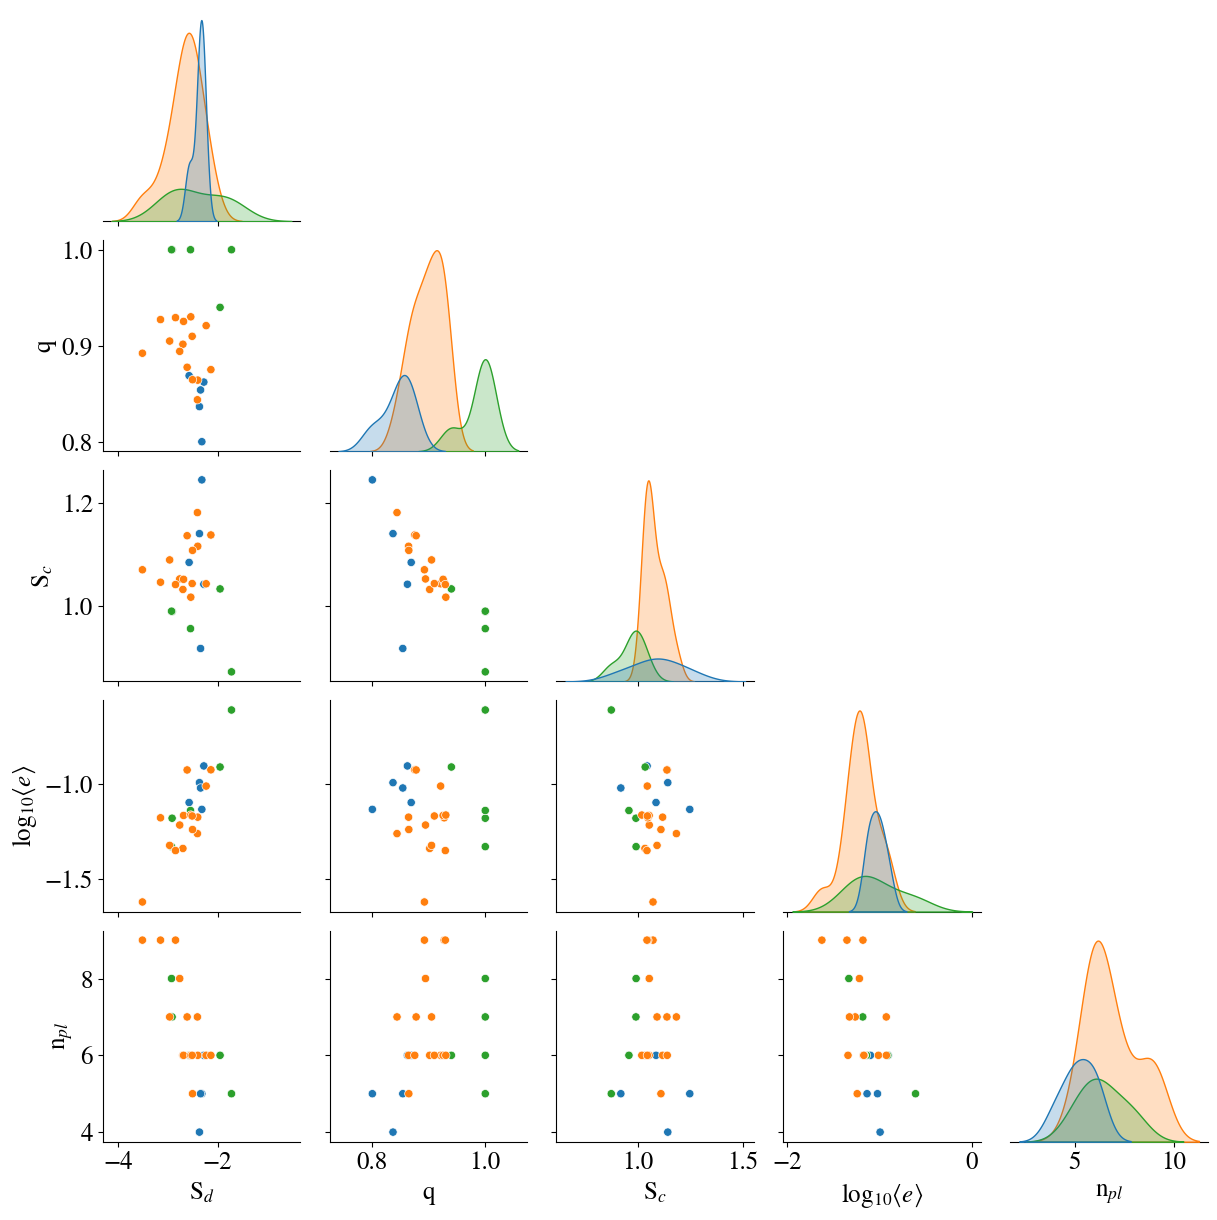
\includegraphics[width=\textwidth]{figures/stip/corner_full_syn_iso.png}
    \caption{Figure caption goes here.\label{fig:corner_full_syn_iso}}
\end{center}
\end{figure*}

In addition to examining the mass and eccentricity distributions, along with the collisional evolution of the simulations, we quantify some global properties of the planetary systems and compare these values between each set of simulations. The first of these quantities $\alpha$, is the total disk mass ratio between the initial and final simulation snapshots. This value quantifies the change in the solid disk mass and is a measure of how much material has been ejected during the giant impact phase. We also measure the mean eccentricity of each planetary system, along with the total number of planets.

In addition, we calculate the radial mass concentration (RMC) $S_{c}$ of each planetary system, which is a measure of how centrally concentrated the solid material is about the star. Following \cite{chambers01}, we define the radial mass concentration statistic as

\begin{equation}\label{eq:rmc}
	S_{c} = \mathrm{max} \left( \frac{\Sigma_{j} m_{j}}{\Sigma_{j} m_{j} \left[ \mathrm{log}_{10} \left( a / a_{j} \right) \right]^{2}} \right),
\end{equation}

\noindent where $a_{j}$ and $m_{j}$ are the semimajor axis and mass of the $j$th planet and $S_{c}$ is the maximum value of the bracketed quantity evaluated over all $a$.

Lastly, we measure the angular momentum deficit (AMD) $S_{d}$ for each planetary system, which is defined as

\begin{equation}\label{eq:amd}
	S_{c} = \frac{\Sigma_{j} m_{j} \sqrt{a_{j} \left( 1 - e_{j}^2 \right)} \mathrm{cos} i_{j} - \Sigma_{j} m_{j} \sqrt{a_{j}}}{\Sigma_{j} m_{j} \sqrt{a_{j}}},
\end{equation}

\noindent \cite{laskar97, chambers01} where $e_{j}$ and $i_{j}$ are the eccentricity and inclination of the $j$th plane. Physically, $S_{c}$ can be thought as the fractional difference between the z-component of the actual total angular momentum of the system and the angular momentum if all of the planets were on circular, non-inclined orbits.

In figure \ref{fig:corner_full_syn_iso}, we show a corner plot highlighting the correlations between these quantities for the full (color), isolation mass (color) and synthetic (color) simulations. (Discuss this plot later)

\begin{figure}
\begin{center}
    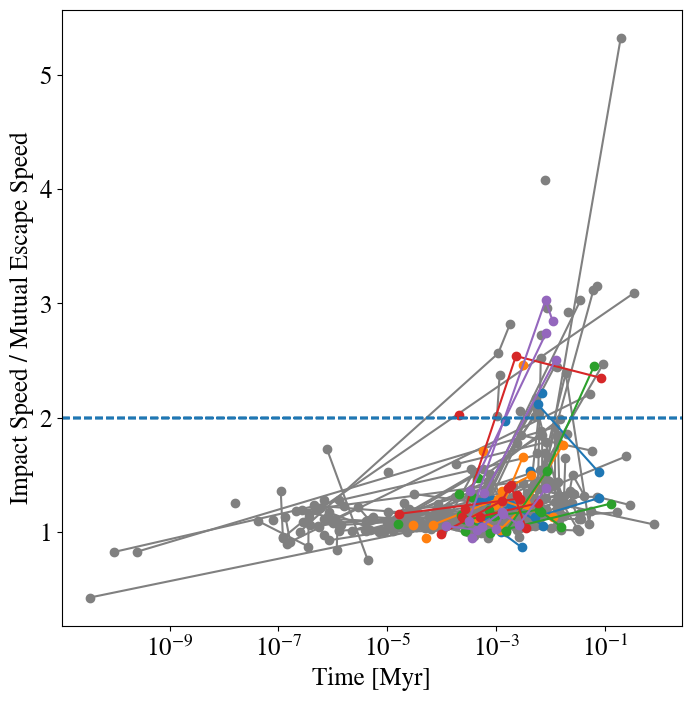
\includegraphics[width=0.5\textwidth]{figures/stip/impact_syn_comp.png}
    \caption{Figure caption goes here.\label{fig:impact_syn_comp}}
\end{center}
\end{figure}

In figure \ref{fig:impact_syn_comp}, we show the timing and impact speed (in units of the mutual escape velocity of the colliding bodies) as a function of time for the full (colored points) and synthetic (gray points) simulations for bodies larger than $0.01 M_{\oplus}$. Subsequent collisions between the same body are connected by lines and the horizontal dashed line at $v_{coll}/v_{mut, esc}$ indicates the speed at which giant impacts should be expected to become destructive \cite{marcus09}. For both the synthetic and full simulations, subsequent collisions speeds begin to ramp up and exceed the destructive limit around $10^{-2}$ Myr. With the exception of many more low-velocity collisions in the synthetic dataset at early times, the two datasets follow a very similar trend on this plot, which is another promising piece of evidence that the data synthesizer is capturing the same dynamical behavior as the full simulations. The cluster of low velocity collisions around $10^{-6}$ Myr in the synthetic simulations is likely due to the early consolidation of protoplanets at the inner edge of the disk seen in figure \ref{fig:full_coll_syn_comp}. However, as we will show in the next figure, this additional phase of giant impacts does not seem to affect the eventual onset of destruction for the innermost planets.

\begin{figure}
\begin{center}
    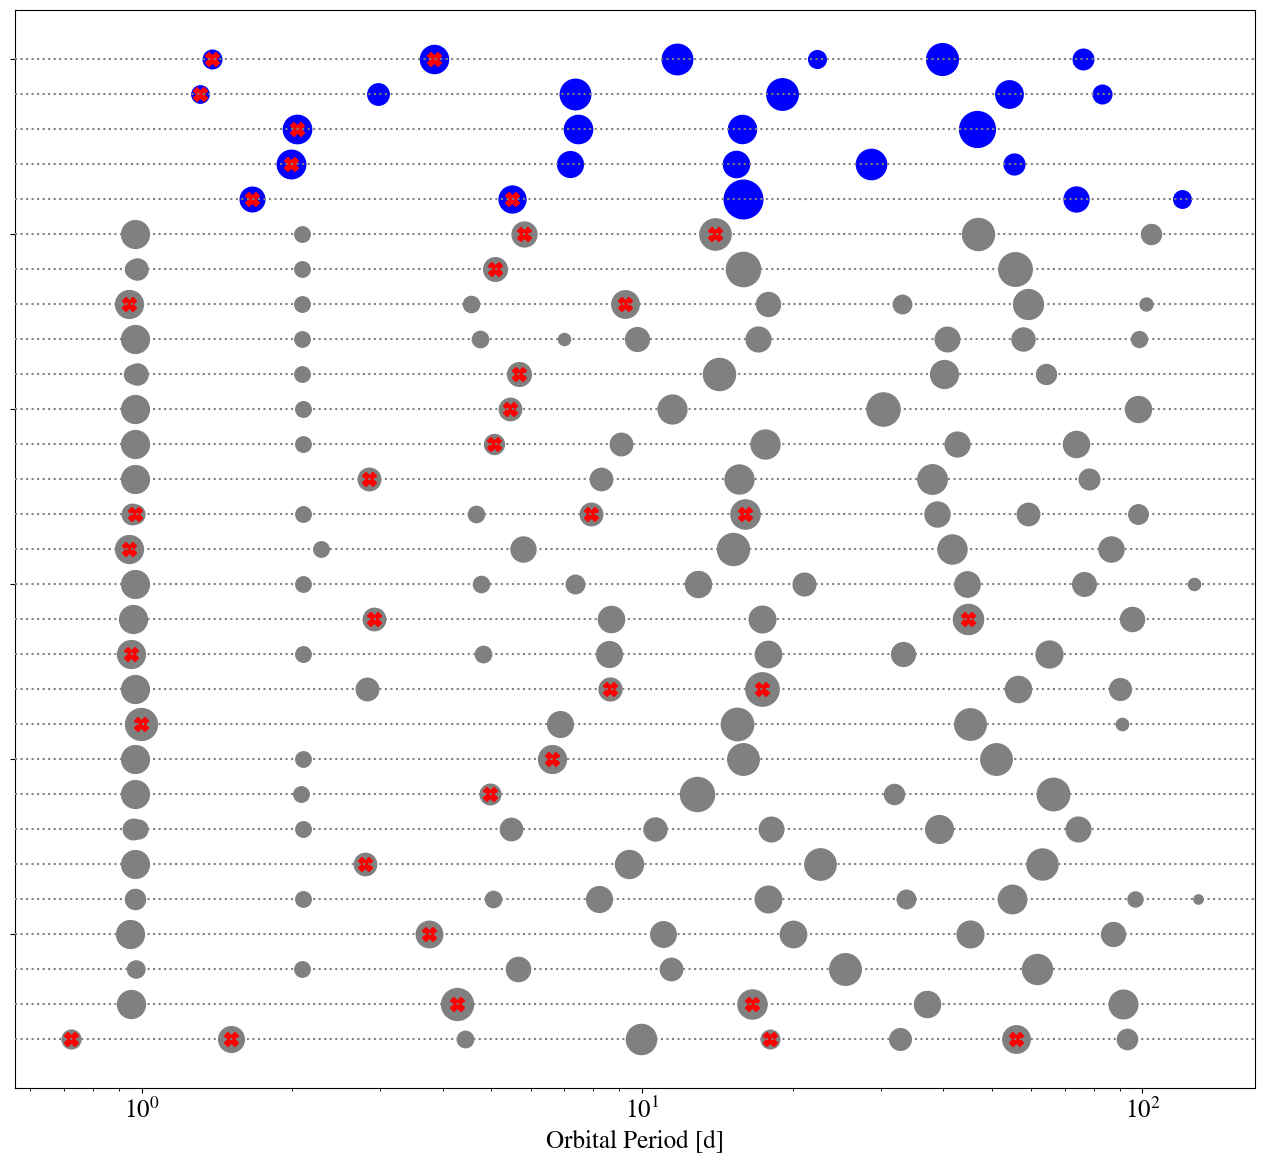
\includegraphics[width=0.5\textwidth]{figures/stip/architectures_syn_comp.png}
    \caption{Figure caption goes here.\label{fig:architectures_syn_comp}}
\end{center}
\end{figure}

\section{Summary and Discussion} \label{sec:discuss}

% Text from NSF proposal:

%With the number of confirmed exoplanets now exceeding 4000, there is now a large enough statistical sample from which to test planet formation theories. The most striking trend in this sample is the prevalence of planets with orbital periods shorter than that of Mercury. Many of these planets come in closely-packed multiples \citep{2014ApJ...790..146F}, known as systems of tightly packed inner planets (STIPs). So far, nearly all STIPs have been found around M stars \citep{2015ApJ...807...45D}. Extending the minimum-mass solar nebula (MMSN) model \citep{1981PThPS..70...35H} down to $\approx$ 0.05 AU, where the inner edge of many protoplanetary disks are thought to be \citep{1997AJ....114..288M} yields several extra Earth masses of material. Explaining why this material is missing from the solar system, but not some exoplanetary systems, is a key question that a complete theory of planet formation must be able to explain.

%There are two categories of theories meant to explain the ubiquity of these compact, short period systems. The first involves the gradual assembly of these worlds as they migrate inwards. Bodies larger than Mars are expected to experience strong torques from the gas disk that drive a substantial amount of migration \citep{1997Icar..126..261W}. Unfortunately, the strength and even direction of this effect is highly uncertain and depends on the detailed physical structure of the disk, along with the specifics of the thermodynamic model used \citep{2010MNRAS.408..876A, 2013A&A...549A.124B}. In addition, many STIPs do not lie in resonant chains, which should be a generic result of convergent migration \citep{2014MNRAS.445..749H}, although dynamical instabilities \citep{2007ApJ...654.1110T, 2019arXiv190709313M} or even turbulence \citep{2011A&A...531A...5P} can potentially disrupt resonant chains after they form.

%Alternatively, these planets may have formed in situ, being constructed only from the local mass budget of the disk. This may be the case for the gaseous envelopes that hot Jupiters attain near the inner edge of the disk \citep{2018ApJ...866L...2B}, although it is not clear if the cores of these worlds also formed locally. Additionally, magnetically driven disk winds, which are especially prevalent around M stars, have been shown to flatten the radial surface density profile, which suppresses type I migration \citep{2018A&A...615A..63O}.

%One of the first simulations of in situ short period terrestrial planet accretion was done by \citet{2007ApJ...669..606R}, who concluded that it was extremely difficult for this process to occur near the habitable zone of M stars. However, the initial conditions used were based off of the MMSN, scaled linearly by the mass of the host star. \citet{2013MNRAS.431.3444C} later showed that the rescaled MMSN tends to underpredict the mass budget of many extrasolar disks. Starting with a much higher surface density, \citet{2012ApJ...751..158H} were able to produce short period Earth-sized planets without invoking migration. A subsequent study by \citet{2014ApJ...795L..15S} argued that applying the MMSN analysis to some exoplanetary systems produced disks that were unphysical, assuming a gas to dust ratio of 1\%. There is no evidence, however that this ratio is universal and there is mounting evidence that shows that this quantity can vary radially \citep{2012ApJ...744..162A, 2014ApJ...788...59W}. It should also be noted that as of yet there are no direct measurements of the surface density profiles of the inner parts of protoplanetary disks. Additionally, the dust masses of disks measured with ALMA have been shown to sometimes underpredict the true values \citep{2019ApJ...878..116P, 2019ApJ...877L..18Z}.

%The question of whether or not in situ formation is viable for STIPs seems to rest largely on what the distribution of planetary embryos looked like that went on to assemble the final configuration of planets. In all of the aforementioned studies, the oligarchic growth model \citep{1998Icar..131..171K, 2000Icar..143...15K} is used to predict the sizes and spacings between the embryos going into the final phase of accretion. \citet{2002ApJ...581..666K} explored the influence of planetesimal orbital distance and surface density profile on the distribution of embryos, but did not extend the search of parameter space down to be of relevance to most STIPs.

%As we will present in a pilot study, runaway and oligarchic growth, which produces a bimodal population of embryos and dynamically hot, difficult to accrete planetesimals, does not appear to operate at short orbital periods. With a colder background population of planetesimals, growth should be more efficient and result in larger embryos. More massive embryos are also less affected by radial drift, which has been cited as a problem with short period in situ formation models \citep{2015MNRAS.448.1751I}. Given the lack of work that has been done on short period planetesimal accretion, along with the subsequent discovery that short period terrestrial worlds are incredibly common, a more careful examination of this phase of growth is warranted. This will place better context on the initial conditions used by recent simulations of short period late stage accretion.
